\documentclass[12pt,a4paper]{amsart}
% ukazi za delo s slovenscino -- izberi kodiranje, ki ti ustreza
\usepackage[english]{babel}
\usepackage[utf8]{inputenc}
%\usepackage[T1]{fontenc}
\usepackage{amsmath,amssymb,amsfonts}
\usepackage{url}
%\usepackage[normalem]{ulem}
\usepackage[dvipsnames,usenames]{color}
\usepackage{caption}
\usepackage{lipsum}
\usepackage{tikz}
\usepackage{xcolor}
\usepackage[linesnumbered,ruled,vlined]{algorithm2e}
\usepackage{geometry}
\usepackage{array}
\usepackage{hyperref}

\usetikzlibrary{graphs}
\usetikzlibrary{graphs.standard}

\makeatletter
\renewcommand\section{\@startsection{section}{1}
  \z@{.5\linespacing\@plus.7\linespacing}{.5\linespacing}
  {\normalfont\scshape\large\centering}}
\renewcommand\subsection{\@startsection{subsection}{2}
  \z@{.5\linespacing\@plus.7\linespacing}{.5\linespacing}
  {\normalfont\scshape}}
\renewcommand\subsubsection{\@startsection{subsubsection}{3}
  \z@{.5\linespacing\@plus.7\linespacing}{-.5em}
  {\normalfont\itshape}}
\makeatother

% ne spreminjaj podatkov, ki vplivajo na obliko strani
\textwidth 15cm
\textheight 24cm
\oddsidemargin.5cm
\evensidemargin.5cm
\topmargin-5mm
\addtolength{\footskip}{10pt}
\pagestyle{plain}
\overfullrule=15pt % oznaci predlogo vrstico


% ukazi za matematicna okolja
\theoremstyle{definition} % tekst napisan pokoncno
\newtheorem{definicija}{Definition}[section]
\newtheorem{primer}[definicija]{Example}
\newtheorem{opomba}[definicija]{Remark}

\renewcommand\endprimer{\hfill$\diamondsuit$}

\theoremstyle{plain} % tekst napisan posevno
\newtheorem{lema}[definicija]{Lemma}
\newtheorem{izrek}[definicija]{Theorem}
\newtheorem{trditev}[definicija]{Statement}
\newtheorem{posledica}[definicija]{Corollary}
\newtheorem{conjecture}[definicija]{Conjecture}


% za stevilske mnozice uporabi naslednje simbole
\newcommand{\R}{\mathbb R}
\newcommand{\N}{\mathbb N}
\newcommand{\Z}{\mathbb Z}
\newcommand{\C}{\mathbb C}
\newcommand{\Q}{\mathbb Q}

% ukaz za slovarsko geslo
\newlength{\odstavek}
\setlength{\odstavek}{\parindent}
\newcommand{\geslo}[2]{\textbf{#1}\hspace*{3mm}\hangindent=\parindent\hangafter=1 #2}

% naslednje ukaze ustrezno popravi
\newcommand{\program}{Financial mathematics} % ime studijskega programa: Matematika/Finančna matematika
\newcommand{\imeavtorja}{Tanja Luštrek, Anej Rozman} % ime avtorja
\newcommand{\imementorja}{Assistant Professor Janoš Vidali} % akademski naziv in ime mentorja
\newcommand{\imesomentorja}{Professor Riste Škrekovski}
\newcommand{\naslovdela}{Rich-Neighbor Edge Colorings}
\newcommand{\letnica}{2023} %letnica diplome

\begin{document}

\thispagestyle{empty}
{\large
\noindent UNIVERSITY OF LJUBLJANA\\[1mm]
FACULTY OF MATHEMATICS AND PHYSICS\\[5mm]
\program\ -- 1st cycle}
\vfill

\begin{center}{\large
\imeavtorja\\[2mm]
{\bf \naslovdela}\\[10mm]
Term Paper in Finance Lab\\[2mm]
Long Presentation\\[1cm]
Advisers: \imementorja, \\ \imesomentorja\\[2mm]}
\end{center}
\vfill

{\large
Ljubljana, \letnica}
\pagebreak

\thispagestyle{empty}
\tableofcontents
\pagebreak

\section{Introduction}

    In this paper we set out to analyse an open conjecture in a modern graph theory problem known as rich-neighbor edge coloring. 

    \begin{definicija}
        In an edge coloring, an edge $e$ is called $rich$ if all edges adjacent to $e$ have different colors. An edge coloring is 
        called a $rich\text{-}neighbor \ edge \ coloring$ if every edge is adjacent to some rich edge.
    \end{definicija}

    \begin{definicija}
        $X'_{rn}(G)$ denotes the smallest number of colors for which there exists a rich-neighbor edge coloring.
    \end{definicija}

    \begin{conjecture}
        For every graph $G$ of maximum degree $\Delta$, $X'_{rn}(G) \leq 2\Delta - 1$ holds.
    \end{conjecture}

    In the paper we focus on analysing the conjecture only for regular graphs. We do this by implementing an integer programming model that finds a rich-neighbor edge coloring for a given graph using the smallest number of colors possible.

    \begin{primer}
    Let's take a look at the Petersen graph and an example of a rich-neighbor edge coloring.\\
    \begin{center}
        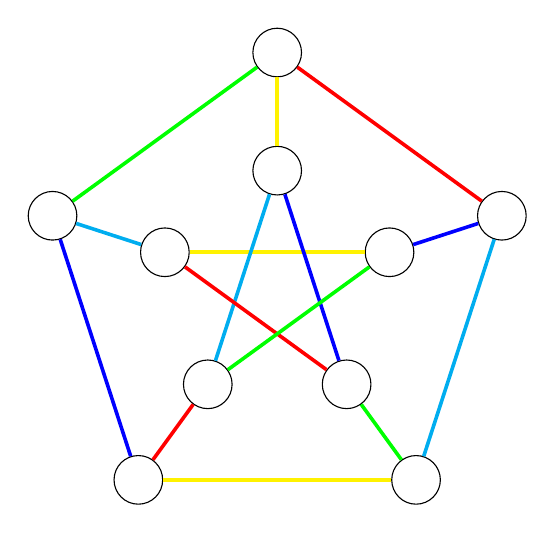
\begin{tikzpicture}[every node/.style={draw,circle, style={text opacity=0}}]
            \graph[clockwise, radius=3cm] {subgraph C_n [n=5,name=A] };
            \graph[clockwise, radius=1.5cm] {subgraph I_n [n=5,name=B] };

            % Define edge colors for the graph
            \draw[yellow, line width=1.3pt] (A 1) -- (B 1);
            \draw[blue, line width=1.3pt] (A 2) -- (B 2);
            \draw[green, line width=1.3pt] (A 3) -- (B 3);
            \draw[red, line width=1.3pt] (A 4) -- (B 4);
            \draw[cyan, line width=1.3pt] (A 5) -- (B 5);
            \draw[red, line width=1.3pt] (A 1) -- (A 2);
            \draw[cyan, line width=1.3pt] (A 2) -- (A 3);
            \draw[yellow, line width=1.3pt] (A 3) -- (A 4);
            \draw[blue, line width=1.3pt] (A 4) -- (A 5);
            \draw[green, line width=1.3pt] (A 5) -- (A 1);
            \draw[yellow, line width=1.3pt] (B 5) -- (B 2);
            \draw[cyan, line width=1.3pt] (B 4) -- (B 1);
            \draw[blue, line width=1.3pt] (B 3) -- (B 1);
            \draw[red, line width=1.3pt] (B 5) -- (B 3);
            \draw[green, line width=1.3pt] (B 4) -- (B 2);
        \end{tikzpicture}\\
    \end{center}
    We can see that for the Petersen graph (which is 3-regular) we can find an appropriate coloring with 5 colors so $X'_{rn} \leq 5 \leq 2 \cdot 3 - 1 = 5$. This shows that the conjecture holds for this graph.
    \end{primer}\\
    \textcolor{white}{i\\ i\\ i\\ i\\ i\\ i\\ i\\ i\\ i\\ i\\ i\\}


\section{Algorithms}

    \subsection{Integer Programming}

        Using SageMath we implement an integer program that finds a rich-neighbor edge coloring for a given graph using the smallest number of colors possible. Writen matematically, our interger program looks like this:\\

        \noindent minimize $t$ \hfill \normalsize{\textcolor{black}{we minimize the number of colors we need}}\\
        %vsoto sm dala do 2delta - 1 prej je bla do k a je to kul???
        \ \ \ subject to $\forall e: \quad \sum_{i=1}^{2\Delta - 1} x_{ei} = 1$ \hfill \normalsize{\textcolor{black}{each edge is exactly one color}}\\

        \ \ \ \ \ \ \ \ \ \ \ $\forall i \ \forall u \ \forall v, w \sim u, v \neq u: \quad x_{uv, i} + x_{uw, i} \leq 1$\\[0.1mm]
        \textcolor{white}{hihi} \hfill \normalsize{\textcolor{black}{edges with the same vertex are a different color}}\\

        \ \ \ \ \ \ \ \ \ \ \ $\forall e \ \forall i: \quad x_{ei} \cdot i \leq t$ \hfill \normalsize{\textcolor{black}{we use less or equal to $t$ colors}}\\

        \ \ \ \ \ \ \ \ \ \ \ $\forall i \ \forall uv \ \forall w \sim u, w \neq v \ \forall z \sim v, z \neq u, w: \quad x_{uw, i} + x_{vz, i} + y_{uv} \leq 2$ \hfill \\[0.1mm]
        \textcolor{white}{hihi} \hfill \normalsize{\textcolor{black}{$uv$ is a rich edge $\Leftrightarrow$ all adjacent edges are a different color}}\\

        \ \ \ \ \ \ \ \ \ \ \ $\forall e: \quad \sum_{f \sim e}y_f \geq 1$ \hfill \normalsize{\textcolor{black}{every edge is adjacent to some rich edge}}\\

        %\ \ \ \ \ \ \ \ \ \ \ \ \ \ $t \geq 2 \Delta - 1$ \hfill \normalsize{\textcolor{black}{we use $\geq 2 \Delta - 1$ colors}}\\

        \ \ \ \ \ \ \ \ \ \ \ $\forall e: \quad 0 \leq y_{e} \leq 1$, $y_{e} \in \Z$\hfill \normalsize{\textcolor{black}{solutions are binary variables}}\\

        \ \ \ \ \ \ \ \ \ \ \ $\forall e \ \forall i: \quad 0 \leq x_{ei} \leq 1$, $x_{ei} \in \Z$,\\

        where
        \begin{align*} x_{ei} = 
            \begin{cases}
                1, \  \text{if edge $e$ is color $i$} \\
                0, \  \text{otherwise}
            \end{cases} \ \ & \text{and} & 
                y_{e} = 
            \begin{cases}
                1, \  \text{if edge $e$ is rich} \\
                0, \  \text{otherwise.}
            \end{cases}
        \end{align*}

        In our implementation of the ILP we fix the number of colors to $2 \Delta - 1$ by adding the following constraint $t = 2\Delta - 1$. We do this since the coloring can't be made with less colors, because every edge has $2 \Delta - 2$ neighboring edges and the edge itself has to be a different color. 
        
        \begin{center}
            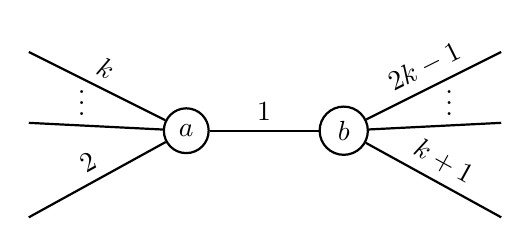
\begin{tikzpicture}[node distance={20mm}, thick, main/.style = {draw, circle}] 
                \node[main] (1) {$a$}; 
                \node[main] (2) [right of=1] {$b$}; 
        
                % sredina
                \draw (1) -- node[midway, above] {1} (2); 
            
                % levo
                \draw (1) -- node[midway, above, sloped] {$k$} ++(-2,1);
                \draw (1) -- node[midway, above, sloped] {2} ++(-2,-1.1);
                %\draw (1) -- node[midway, above left, sloped] {3} ++(-2,-0.3);
                \draw (1) -- node[above left]{\vdots} ++(-2, 0.1);
            
                %desno
                \draw (2) -- node[midway, above, sloped] {$2k-1$} ++(2,1);
                \draw (2) -- node[midway, above, sloped] {$k+1$} ++(2,-1.1);
                %\draw (2) -- node[midway, above right, sloped] {$k+2$} ++(2,-0.3);
                \draw (2) -- node[above right]{\vdots} ++(2, 0.1);
        
            \end{tikzpicture}
        \end{center}

        
        And since any coloring with more than $2\Delta - 1$ colors does not satisfy the conjecture, we only check if the program has a solution that satisfies all the constraints. In theory this doesn't make the program faster, but in our practice tests it did make a significant differnece.\\

        \pagebreak
        Our actual implementation of the ILP is demonstrated in the following code.


        \begin{algorithm}%[!htbp]
            \caption{richNeighbor}\label{algo:richNeighbor}
            \LinesNumberedHidden
            \DontPrintSemicolon
            %\SetAlgoNlRelativeSize{0}
            %\SetAlgoNlRelativeSize{-1}
            %\SetAlgoNlRelativeSize{1}
            \SetKwInput{KwInput}{Input}
            \SetKwInput{KwOutput}{Output}

            \SetKwFunction{FMain}{richNeighbor}

            \KwInput{graph $G$}
            \KwOutput{colors of edges $colors$, rich edges $richEdges$}

            $p \gets$ MixedIntegerLinearProgram(maximization = False)\;
            $x \gets p.\text{new\_variable(binary = True)}$\;
            $y \gets p.\text{new\_variable(binary = True)}$\;
            $t \gets p.\text{new\_variable(integer = True)}$\;
            $p.\text{set\_objective}(t[0])$\;

            $maxCol \gets 2 \cdot G.degree()[0] - 1$\;

            $p.\text{add\_constraint}(t[0] = \text{maxCol})$\;

            \For{$e$ in $G.edges(\text{labels} = \text{False})$}{
                $p.\text{add\_constraint}(\sum_{i=1}^{maxCol} x[\text{Set}(e), i] = 1)$\;
            }

            \For{$(u,v)$ in $G.edges(\text{labels} = \text{False})$}{
                $p.\text{add\_constraint}(\sum_{j \in G[u]} y[\text{Set}((u, j))] + \sum_{l \in G[v]} y[\text{Set}((l, v))] - 2y[\text{Set}((u, v))] \geq 1)$\;
            }

            \For{$e$ in $G.edges(\text{labels} = \text{False})$}{
                \For{$i$ in $1$ to $\text{maxCol}$}{
                    $p.\text{add\_constraint}(i \cdot x[\text{Set}(e), i] \leq t[0])$\;
                }
            }

            \For{$i$ in $1$ to $\text{maxCol}$}{
                \For{$(u,v)$ in $G.edges(\text{labels} = \text{False})$}{
                    \For{$w$ in $G[u]$}{
                        \If{$w = v$}{
                            \textbf{continue}\;
                        }
                        $p.\text{add\_constraint}(x[\text{Set}((u, v)), i] + x[\text{Set}((u, w)), i] \leq 1)$\;
                    }
                    \For{$z$ in $G[v]$}{
                        \If{$z = u$}{
                            \textbf{continue}\;
                        }
                        $p.\text{add\_constraint}(x[\text{Set}((u, v)), i] + x[\text{Set}((v, z)), i] \leq 1)$\;
                    }
                }
            }

            \For{$(u, v)$ in $G.edges(\text{labels}=False)$}{
                \For{$w$ in $G.neighbors(u)$}{
                    \For{$z$ in $G.neighbors(v)$}{
                        \If{$w = v$ or $z = u$}{
                            \textbf{continue}\;
                        }
                        \For{$i$ in $1$ to $\text{maxCol}$}{
                            $p.\text{add\_constraint}(x[\text{Set}((u, w)), i] + x[\text{Set}((v, z)), i] + y[\text{Set}((u, v))] \leq 2)$\;
                        }
                    }
                }
            }

            %\Try{
            %    $p.solve()$\;
            %    $colors \gets p.get\_values(x)$\;
            %    $richEdges \gets p.get\_values(y)$\;
            %}
            %\Catch{ValueError}{
            %    $\text{print}(\text{f'BINGO! The graph }{G}\text{ doesn't have a rich-neighbor edge coloring! \n' + f'Edges: }{G.edges()} \text{; \n' + f'Adjacency matrix: }{G.adjacency\_matrix()} \text{; \n' + f'Neighbors: }{G.neighbors()})$\;
            %    \Return \text{False, False}\;
            %}
            %
            \Return $colors$, $richEdges$\;
            \end{algorithm}

            \pagebreak

            \begin{primer}
                Using the \texttt{richNeighbor} algorithm on the Petersen graph gives us the following output.\\*

                \begin{align*}
                    colors = \{ & (\{0, 1\}, 1): 0.0, (\{0, 1\}, 2): 0.0, (\{0, 1\}, 3): 0.0, (\{0, 1\}, 4): 0.0,\\
                                & (\{0, 1\}, 5): 1.0, (\{0, 4\}, 1): 0.0, (\{0, 4\}, 2): 0.0, (\{0, 4\}, 3): 1.0,\\
                                & \cdots \\
                                & (\{9, 6\}, 3): 0.0, (\{9, 6\}, 4): 0.0, (\{9, 6\}, 5): 0.0, (\{9, 7\}, 1): 0.0,\\
                                & (\{9, 7\}, 2): 0.0, (\{9, 7\}, 3): 0.0, (\{9, 7\}, 4): 1.0, (\{9, 7\}, 5): 0.0\}
                \end{align*}

                \begin{align*}
                    richEdges = \{& \{0, 1\}: 1.0, \{0, 4\}: 0.0, \{0, 5\}: 0.0, \{1, 2\}: 1.0, \{1, 6\}: 0.0,\\
                                  & \{3, 4\}: 0.0, \{9, 4\}: 1.0, \{5, 7\}: 0.0, \{8, 5\}: 1.0, \{2, 3\}: 1.0,\\
                                  & \{2, 7\}: 0.0, \{8, 6\}: 0.0, \{9, 6\}: 0.0, \{8, 3\}: 1.0, \{9, 7\}: 1.0\}\\
                \end{align*}

                \noindent Both $colors$ and $richEdges$ are dictionaries and their key-value pairs are structured like

                \begin{align*}
                    (e, i):
                    \begin{cases}
                        1.0, \  \text{if edge $e$ is color $i$} \\
                        0.0, \  \text{otherwise}
                    \end{cases} & \text{and} & 
                    e:
                    \begin{cases}
                        1.0, \  \text{if edge $e$ is rich} \\
                        0.0, \  \text{otherwise.}
                    \end{cases}
                \end{align*}

            \end{primer}    

    \subsection{Iterative Algorithm}
            
        We debated implementing an iterative algorithm that finds a rich neighbor edge coloring, but we were not able to come up with anything that runs in polynomial time. From \cite{10.1007/978-3-642-95322-4_17} we know that integer linear programs are NP-complete problems, so it did't make much sense implementing another slow algorithm, since it wouldn't make much of a difference in the number of graphs we would be able to check.
        \textcolor{white}{i\\ i\\ i\\ i\\ i\\ i\\ i\\ i\\ i\\ i\\ i\\ i\\ i\\ i\\ i\\ i\\}
\pagebreak
\section{Complete Search}

    As illustrated in Table \ref{table:1}, the number of $k$-regular graphs on $n$ vertices grows exponentially with $n$. This poses a computational challenge, as checking all graphs becomes impossible for larger values of n. However, we can still check all graphs for smaller values of n up to 15.

    \begin{table}[!htbp]
        \centering
        \begin{tabular}{|c|c|c|c|c|}
            \hline
            Vertices & Degree 4 & Degree 5 & Degree 6 & Degree 7 \\
            \hline
            5 & 1 & 0 & 0 & 0 \\
            6 & 1 & 1 & 0 & 0 \\
            7 & 2 & 0 & 1 & 0 \\
            8 & 6 & 3 & 1 & 1 \\
            9 & 16 & 0 & 4 & 0 \\
            10 & 59 & 60 & 21 & 5 \\
            11 & 265 & 0 & 266 & 0 \\
            12 & 1544 & 7848 & 7849 & 1547 \\
            13 & 10778 & 0 & 367860 & 0 \\
            14 & 88168 & 3459383 & 21609300 & 21609301 \\
            15 & 805491 & 0 & 1470293675 & 0 \\
            16 & 8037418 & 2585136675 & 113314233808 & 733351105934 \\
            \hline
        \end{tabular}
        \caption{Number of $k$-regular graphs on $n$ vertices \cite{meringer1999fast}
        }
        \label{table:1}
    \end{table}
    \subsection{Graph Generation}
        Graphs for the complete search were taken from a collection of files, provided by Professor Škrekovski. The files contain all $k$-regular graphs on $n$ vertices up to 15 vertices, since the number of graphs beyond that is too much to handle.\\

\section{Random Search}

    In addition to examining the hypothesis for smaller graphs, we were also interested in checking if the conjecture holds for larger graphs. The challenge here is testing all possible colorings in graphs with many vertices.
    Recognizing the enormity of this task, a random search algorithm seemed like a natural continuation of our problem. Here we opted for a modification approach.\\

    We start with a random graph and use our ILP to check if the conjecture holds for it. Then, we modify the graph in a way that preserves its regularity and connectedness. We repeat this process indefinitely, or actually, until we stop our program. We know that if a rich-neighbor edge coloring exists in a given graph, there is a higher probability that it also exists in similar graphs. Therefore, on every iteration, we keep a small probability that we generate a completely new random graph and start again.\\

    \textcolor{white}{i\\ i\\ i\\ i\\}
    \pagebreak

    Written below is the algorithm \texttt{tweak} for modifying graphs. First it selects two random edges and deletes them. Then it generates a random number $p$ from $[0, 1)$ and based on the value of $p$ it adds back two different edges in one of two possible ways that preserve the regularity of the graph. Since there is a chance that the newly formed graph is not connected, we check for that and if it is not, we restart the process until we get a connected graph.\\
    
    \begin{algorithm}[!htbp]
        \caption{tweak}\label{algo:tweakGraph}
        \LinesNumberedHidden
        \DontPrintSemicolon
        %\SetAlgoNlRelativeSize{0}
        %\SetAlgoNlRelativeSize{-1}
        %\SetAlgoNlRelativeSize{1}
        \SetKwInput{KwInput}{Input}
        \SetKwInput{KwOutput}{Output}
        
        \SetKwFunction{FTweakGraph}{tweakGraph}
        
        \KwInput{graph $G$}
        \KwOutput{tweaked graph $T$}
        

            $T \gets \text{graph.copy()}$\;
            
            $e_1 \gets T.\text{random\_edge()}$\;
            $u_1, v_1, \gets e_1$\;
            $T.\text{delete\_edge}(e_1)$\;
            
            $e_2 \gets T.\text{random\_edge()}$\;
            $u_2, v_2,  \gets e_2$\;
            $T.\text{delete\_edge}(e_2)$\;
        
            $p \gets \text{random}()$\;
            \If{$p < 0.5$}{
                $T.\text{add\_edge}(u_1, u_2)$\;
                $T.\text{add\_edge}(v_1, v_2)$\;
            }\Else{
                $T.\text{add\_edge}(u_1, v_2)$\;
                $T.\text{add\_edge}(v_1, u_2)$\;
            }
            
            \If{\text{not $T$.is\_connected()}}{
                \Return \text{tweak}($G$)\;
            }
            
            \Return $T$\;
        \end{algorithm}

    \subsection{Graph Generation}
        Since we only need one graph to start our iterative process, we can generate it randomly, using the built-in SageMath function \texttt{graphs.RandomRegular}.

\section{Checking the Coloring} 
    In order to make sure that our ILP implentation is without fault, we also implement the functions \texttt{checkColoring} and \texttt{checkRichness} which check if our program always returns a proper coloring, and if the coloring is actually a rich-neighbor edge coloring.\\
    \textcolor{white}{i\\ i\\ i\\}
    \pagebreak
    
    \texttt{checkColoring} takes a graph $G$ and the output $colors$ of our ILP. It iterates over\* each vertex in the graph, checks all edges adjacent to it, and returns false if it finds two or more edges with the same color.\\

    \begin{algorithm}%[!htbp]
        \caption{checkColoring}\label{algo:checkColoring}
        \LinesNumberedHidden
        \DontPrintSemicolon
        %\SetAlgoNlRelativeSize{0}
        %\SetAlgoNlRelativeSize{-1}
        %\SetAlgoNlRelativeSize{1}
        \SetKwInput{KwInput}{Input}
        \SetKwInput{KwOutput}{Output}

        \SetKwFunction{FCheckColoring}{checkColoring}

        \KwInput{graph $G$, colors of edges $coloring$}
        \KwOutput{Boolean indicating proper coloring}

        \For{$v$ in $G.vertices()$}{
            $col \gets \text{set()}$\;
            \For{$w$ in $G.neighbors(v)$}{
                \For{$i$ in $range(1, 2 \cdot G.degree()[0])$}{
                    \If{$coloring[(\text{Set}((v, w)), i)] = 1$}{
                        $col.\text{add}(i)$\;
                }
                }
            }
            \If{$\text{len}(col) \neq \text{len}(G.neighbors(v))$}{
                \Return \text{False}\;
            }
        }
        \Return \text{True}\;
    \end{algorithm}

    \texttt{checkRichness} takes a graph $G$ and the output $richEdges$ of our ILP. It iterates over each edge in the graph, checks all edges adjacent to it, and returns false if it doesn't find a rich edge.\\

    \begin{algorithm}[!htbp]
        \caption{checkRichness}\label{algo:checkRichness}
        \LinesNumberedHidden
        \DontPrintSemicolon
        %\SetAlgoNlRelativeSize{0}
        %\SetAlgoNlRelativeSize{-1}
        %\SetAlgoNlRelativeSize{1}
        \SetKwInput{KwInput}{Input}
        \SetKwInput{KwOutput}{Output}
        
        \SetKwFunction{FCheckRichness}{checkRichness}
        
        \KwInput{graph $G$, rich edges $richEdges$}
        \KwOutput{Boolean indicating proper rich-neighbor edge coloring}
        
        \For{$(u, v)$ in $G.edges(labels = False)$}{
            $S \gets 0$\;
            \For{$w$ in $G.neighbors(u)$}{
                \If{$w = v$}{
                    $S \gets S + richEdges[\text{Set}((u, w))]$\;
                }
            }
            \For{$z$ in $G.neighbors(v)$}{
                \If{$z = u$}{
                    $S \gets S + richEdges[\text{Set}((v, z))]$\;
                }
            }
            \If{$S = 0$}{
                \Return \text{False}\;
            }
        }
        \Return \text{True}\;
    \end{algorithm}

\pagebreak

\section{Findings}
    With the help of Professor Riste Škrekovski, we were able to use external servers to run our algorithms for an extended period of time. We ran a complete search for all regular graphs up to 15 vertices and a random search for regular graphs with 16 vertices or more. The output of our scripts can be seen in the folders \texttt{Complete} and \texttt{Random} in our GitHub repository at \href{https://github.com/anejrozman/Rich-neighbour-edge-coloring}{github/anejrozman}. Table \ref{table:2} shows the number of checked graphs using the random search algorithm for certain classes of graphs.

    \begin{table}[!htbp]
        \begin{tabular}{|c|c|c|c|c|c|}
        \hline
        Degree \textbackslash Vertices & 16            & 17            & 18            & 19     & 20            \\ \hline
        4                              & 216190        & 344180        & 199300        & 321970 & 182260        \\
        5                              & 97340         & /             & 88420         & /      & 81390         \\
        6                              & 49220         & 87710         & 44210         & 79790  & 40390         \\
        7                              & 22500         & /             & 19430         & /      & 18230         \\
        8                              & 6860          & 13910         & 5990          & 12310  & 5270          \\
        9                              & 3530          & /             & 2970          & /      & 2570          \\
        10                             & 1830          & 760           & 50            & 2920   & 1280          \\
        11                             & 70            & /             & 220           & /      & 90            \\
        12                             & \textless{}10 & \textless{}10 & \textless{}10 & 10     & \textless{}10 \\ \hline
        \end{tabular}
        \caption{Number of checked graphs with random search}
        \label{table:2}
    \end{table}
    
    \noindent We can clearly see that our ILP slows down significantly with the regularity of the graphs. This makes intuitive sense since the number of constraints that we have to solve is $\mathcal{O}(k^4n)$ where $k$ is the regularity and $n$ is the number of vertices in the graph we are using our ILP on to find a rich-neighbor edge coloring.\\
    
    \subsection{Problems}
    When going through the complete search file outputs we noticed that each file stopped at 100-th iteration and found that it had a minor bug. We ran it again on our computer and checked all regular graphs up to 13 vertices instead of 15 because the task was to intense for a personal computer.\\

    \subsection{Conclusion}
    We can confirm that every graph that was checked by our algorithm satisfies the conjecture, so based on this it seems likely that the conjecture could hold for all regular graphs. However, we can't be sure of this since, if a counterexample exists it could quite possibly be a very large graph that is very unlikely to be found by any of our algorithms.

    \textcolor{white}{i\\ i\\ i\\ i\\ i\\ i\\}
\pagebreak
\bibliographystyle{plain}
\bibliography{lit}

\end{document}